\documentclass{article}
\usepackage{tikz}

\begin{document}

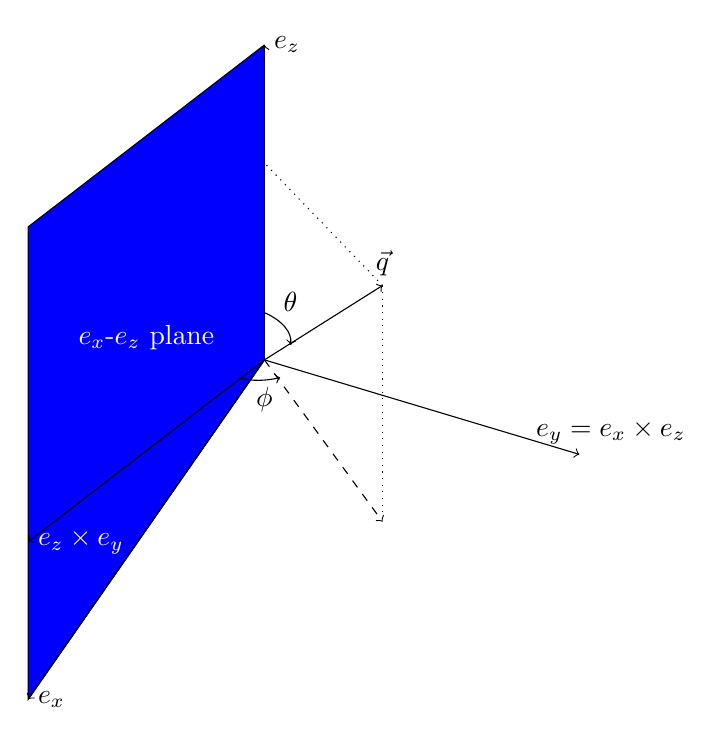
\begin{tikzpicture}[x={(-5mm,-3.85mm)},z={(0,1cm)},y={(1cm,-.3cm)}]
  \draw [fill=blue,text=white] (0,0,0)--(6,0,-2)--(6,0,4)--(0,0,4) node [above,xshift=-1.5cm,yshift=-4cm] {$e_x$-$e_z$ plane};

  \draw [->] (0,0) -- (6,0,-2) node [right] {$e_x$};
  \draw [->] (0,0) -- (0,4,0) node [above,xshift=0.4cm] {$e_y = e_x \times e_z$};
  \draw [->] (0,0) -- (0,0,4) node [right] {$e_z$};

  \draw [->,text=white] (0,0) -- (6,0,0) node [right] {$e_z \times e_y$};

  \draw [dotted] (3,3,3) -- (0,0,2.5);

  \draw [->] (0,0,0) -- (3,3,3) node [above] {$\vec{q}$};
  \draw [dotted] (3,3,3) -- (3,3,0);
  \draw [dashed,->] (0,0,0) -- (3,3,0);


  \draw [->] (0,0,0.6) arc [start angle=170,end angle=120,x radius=1.2,y radius=0.9] node [above,yshift=0.3cm] {$\theta{}$};
  \draw [->] (0.6,0,0) arc [start angle=0,end angle=45,x radius=1,y radius=0.5] node [below,xshift=-0.2cm] {$\phi{}$};

\end{tikzpicture}

\end{document}
